\documentclass[main_conf.tex]{subfiles}

\begin{document}

Las plantas de fabricación de mallas metálicas usan máquinas de
confección de hebras metálicas de diferentes grosores y
longitudes. Estas máquinas no suelen poseer sistema
automatizado, solo están los controles On/Off manual (ver Fig.
\ref{maquina_a_automatizar}, por lo cual la medición de longitud
de cada hebra es manual, lenta y con grandes pérdidas. El proceso
de automatización consiste en reducir al máximo el error de medición
para así reducir la merma y reducir costos de producción. Así mismo,
este sistema será fabricado con materiales de bajo costo y de fácil
obtención en el mercado local.

\begin{figure}[h]
  \centering
  %\includegraphics[width=2.5in]{../img/maquina_a_automatizar.jpg}
  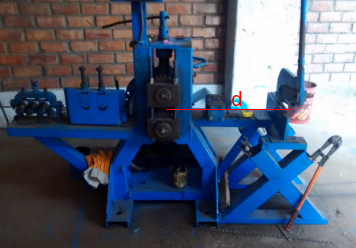
\includegraphics[width=2.5in]{../img/distancia_inicial.png}
  \caption{Rodillo con disco para encoder relativo}
  \label{maquina_a_automatizar}
\end{figure}

\subsection{Descripción de la máquina}
Cuentan con un par de ejes en los cuales se empotran dos ruedas dentadas
del mismo tamaño y mismo número de dientes.

\subsection{Descripción de la solución}
Se construye un módulo de

Se introduce dos rodillos que presionan la hebra generada. Producto de
la fricción, los rodillos giran. Uno de estos es conectado a un disco
encoder con el cual se estima la longitud de la hebra en proceso.

Se usa un Arduino Nano para adquirir las señales del encoder,



\end{document}
